\documentclass[12pt, twoside]{article}
\usepackage[francais]{babel}
\usepackage[T1]{fontenc}
\usepackage[latin1]{inputenc}
\usepackage[left=5mm, right=5mm, top=5mm, bottom=5mm]{geometry}
\usepackage{float}
\usepackage{graphicx}
\usepackage{array}
\usepackage{multirow}
\usepackage{amsmath,amssymb,mathrsfs}
\usepackage{textcomp}
\pagestyle{empty}
\usepackage{soul}
\begin{document} 


\begin{center}
{\fbox{$2^{de}5$ \qquad \qquad \textbf{\Large{Devoir surveill� 7}}
\qquad \qquad 05/06/2009}}
\end{center}


\bigskip

\textit{La deuxi�me feuille est � compl�ter (exercices 2,3 et 4) et � rendre.}

\medskip

\textbf{Exercice 1:}
Un professeur a corrig� les notes de ces �l�ves en 3 fois. Il leur donne les
informations suivantes:

\begin{itemize}
  \item [$\bullet$] $1^{er}$ lot: 12 copies, moyenne 11,2
  \item [$\bullet$] $2^{eme}$ lot: 9 copies, moyenne 10,3
  \item [$\bullet$] $3^{eme}$ lot: 14 copies, moyenne 10,7
\end{itemize}


\begin{enumerate}
  \item Quelle est la moyenne de l'ensemble de la classe?
  \item Trouvant ce devoir difficile, il d�cide de r�hausser toutes les notes.
Il h�site entre augmenter toutes les notes d'un point ou remonter
toutes les notes de 10 \%. Calculer dans les deux cas la moyenne obtenue pour
l'ensemble de la classe. 
\end{enumerate}

\bigskip


\textbf{Exercice 2:}
Le directeur d'un salon de coiffure fait une �tude sur un �chantillon de 72
clients pour conna�tre le temps d'attente moyen des clients. Il obtient les
r�sultats suivants:

\begin{center}
\begin{tabular}{|c|c|c|c|c|}
\hline
Temps (en min)& [0;5[ & [5;15[ & [15;30[ & [30; 60[ \\
\hline
Effectifs & 19 & 26 & 18 & 9 \\
\hline
\end{tabular}
\end{center}

\begin{enumerate}
  \item Selon vous, quel est l'int�r�t de ce sondage pour le directeur?
  \item Repr�senter ces donn�es sous forme d'histogrammes (sur la deuxi�me
  feuille).
  \item Calculer la m�diane et la repr�senter graphiquement.
  
\end{enumerate}

\bigskip

\textbf{Exercice 3:} Les repr�sentations graphiques sont sur la deuxi�me
feuille.


  Soit $f(x)= (x-3)^{2}-1$  et $h(x)=-2x+4$ deux fonctions d�finies sur
  $\mathbb{R}$.

\begin{enumerate}
    \item Parmi les quatre repr�sentations graphiques, retrouver celles des
    fonctions $f$ et $h$. Justifier votre choix.
    \item Dresser le tableau de variation de $f$.
    \item D�montrer par le calcul le sens de variations de $f$ sur $]-\infty;
    3]$.
    \item R�soudre graphiquement $f(x)=h(x)$.
    \item  BONUS: R�soudre alg�briquement $f(x)=h(x)$.


\end{enumerate}


\bigskip

\textbf{Exercice 4:} 

Soient A un point du plan et $\vec{u}$ et $\vec{v}$ deux vecteurs.

\begin{enumerate}
  \item Construire (sur la feuille 2) le point $B$ tel que
  $\overrightarrow{AB}=\vec{u}$.
  \item Construire  le point $C$ tel que
  $\overrightarrow{AC}=\vec{v}$.  
  \item  Construire le point $N$ tel que
  $\overrightarrow{AN}=\dfrac{3}{2} \overrightarrow{AB}+\overrightarrow{AC}$.  
  \item Soit $P$  le point du plan d�fini par $3 \overrightarrow{PB}+2
  \overrightarrow{PC}=\vec{0}$. D�montrer que
  $\overrightarrow{BP}=\dfrac{2}{5} \overrightarrow{BC}$. Placer $P$.
  
  \item    
  
  \begin{enumerate}
    \item Ecrire $\overrightarrow{AN}$ en fonction de $\vec{u}$ et $\vec{v}$.
    \item Ecrire $\overrightarrow{AP}$ en fonction de $\vec{u}$ et $\vec{v}$.
    \item Montrer que $A$, $P$ et $N$ sont align�s.
\end{enumerate}
\end{enumerate}
\pagebreak




NOM:  \quad \quad \quad \quad  \quad \quad \quad \quad \quad  \quad \quad
\quad PRENOM:

\enskip

\textbf{Exercice 2}

\begin{center}
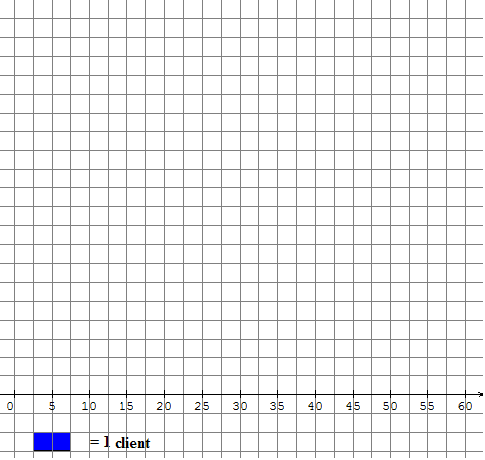
\includegraphics[width=90mm]{images/histo.png}
\end{center} 



\textbf{Exercice 3}

\begin{center}
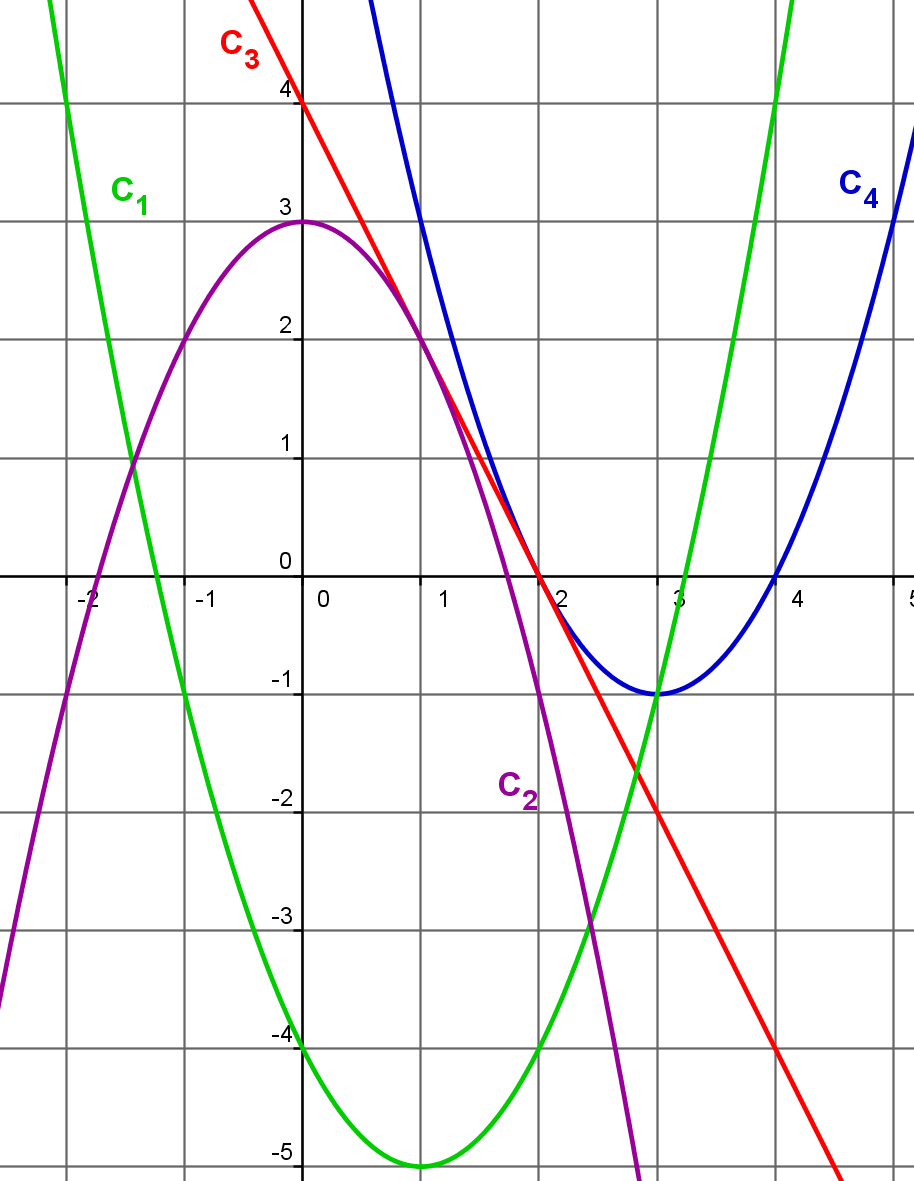
\includegraphics[width=82mm]{images/fonctions.png}
\end{center} 


\textbf{Exercice 4}

\begin{center}
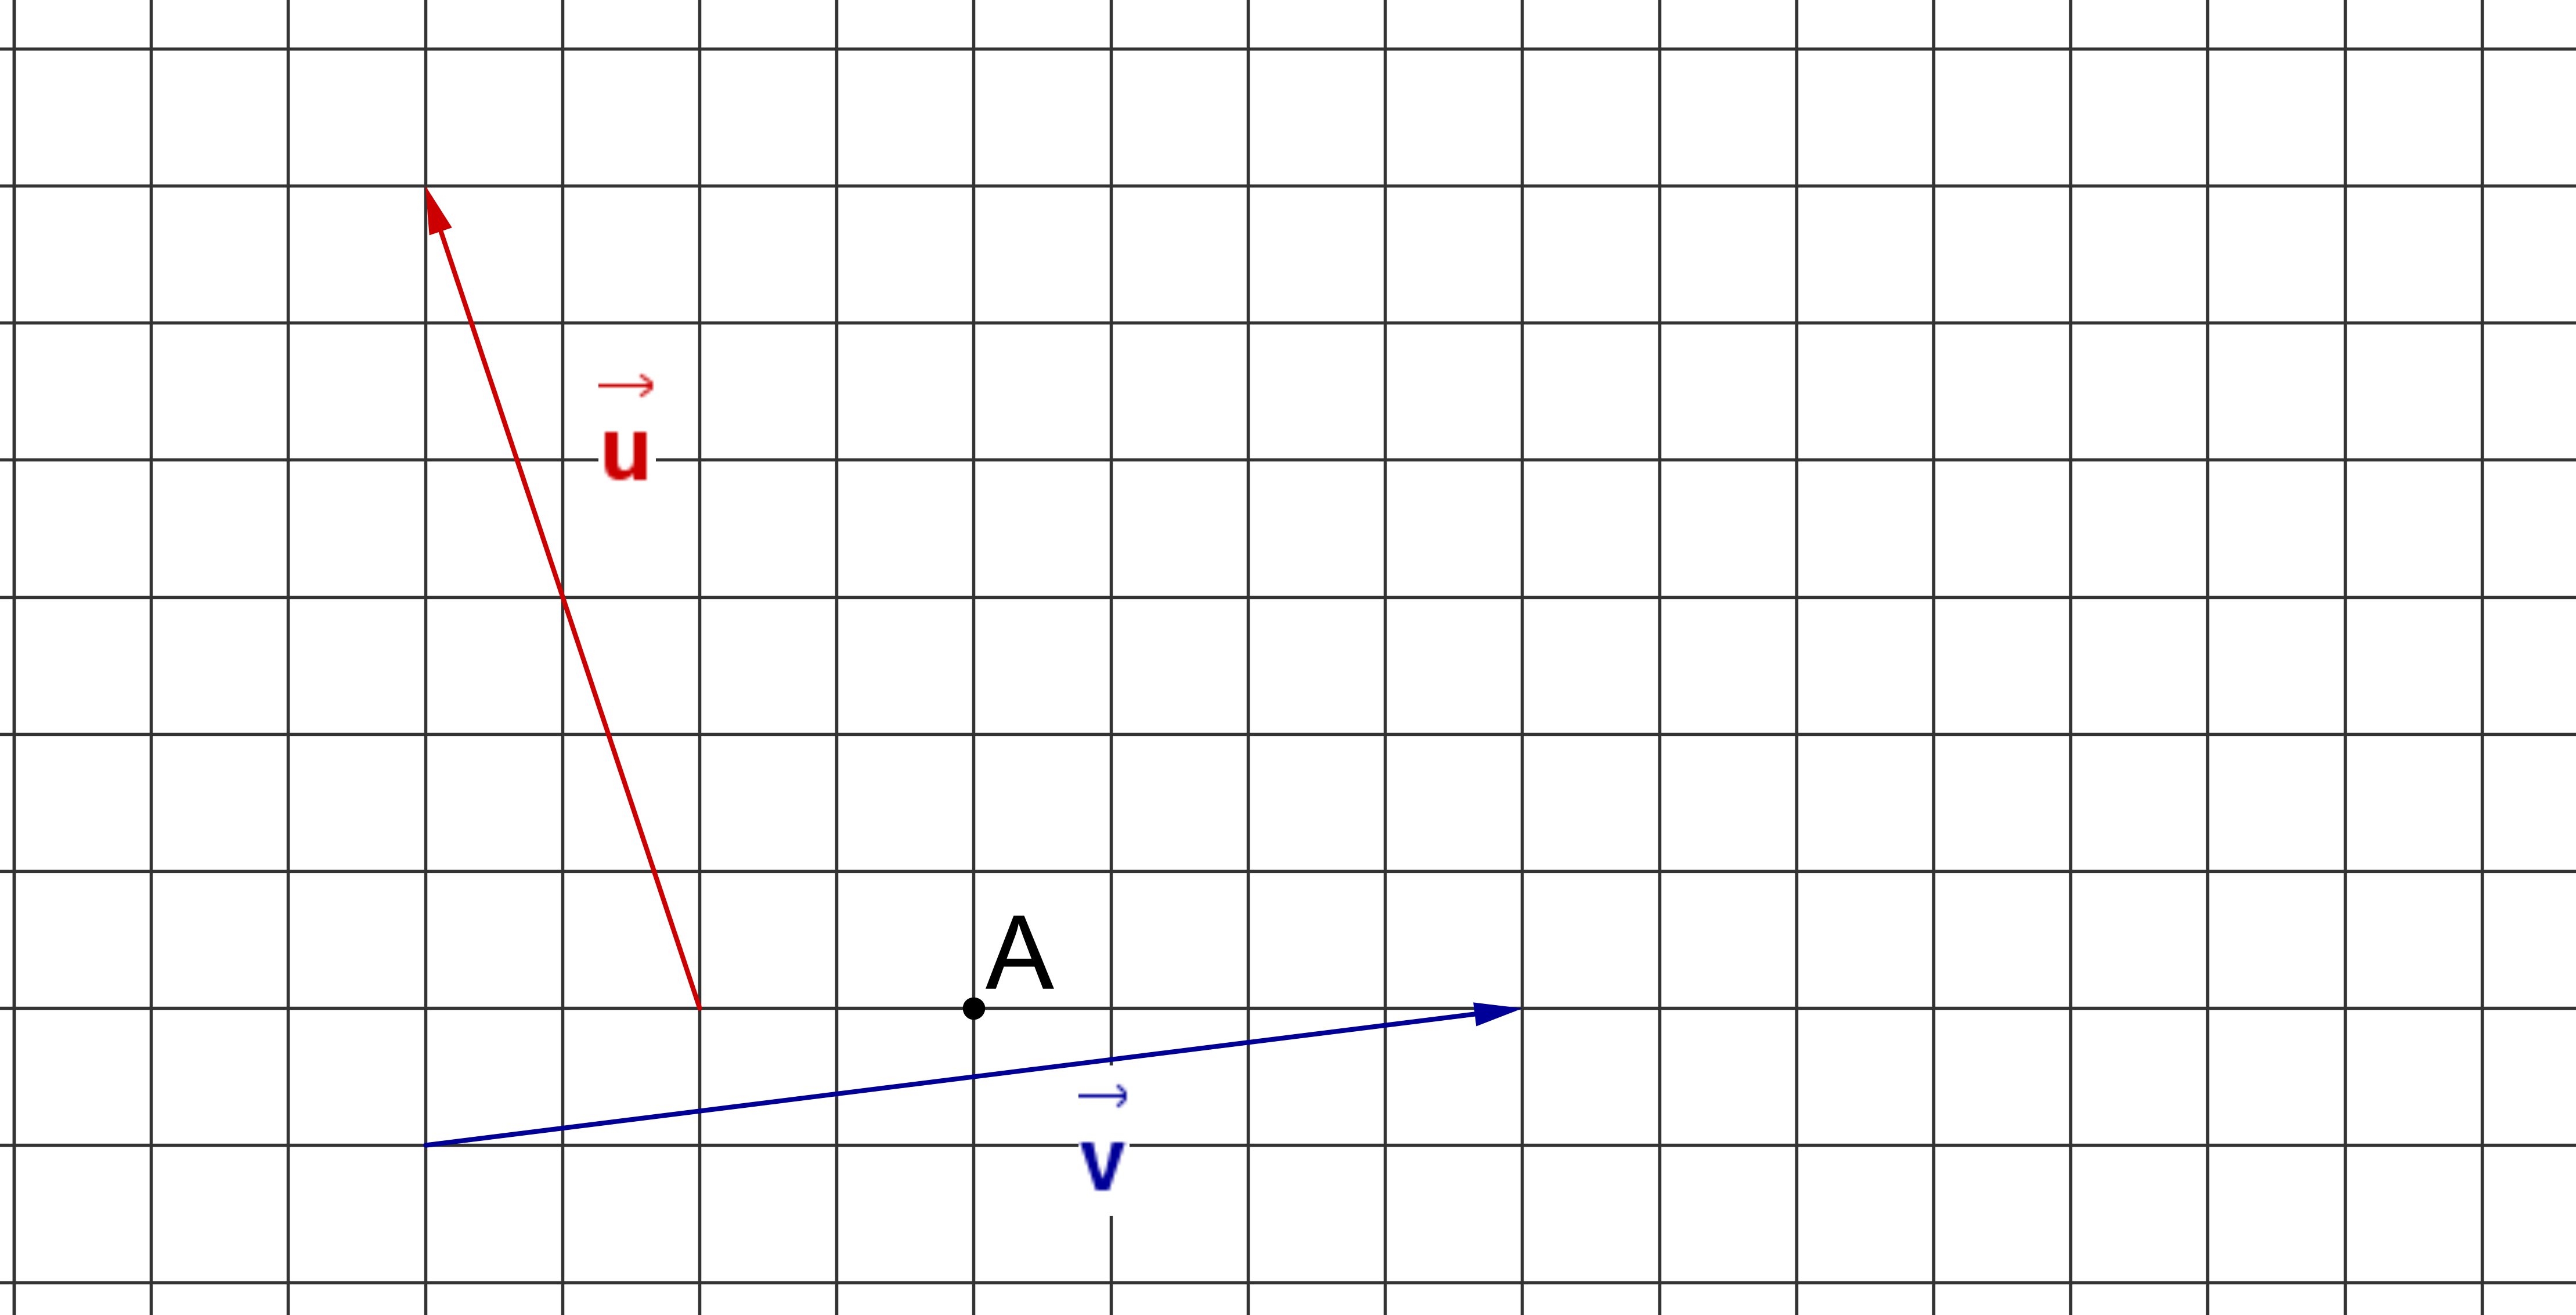
\includegraphics[width=78mm]{images/vecteurs.png} 
\end{center} 


 




\end{document}
